
After \cref{sec:single_shot_classification} we should have a working qubit, fairly calibrated.
But still, we are not taking the most out of it.
In particular, we never really calibrated the readout pulse.
This is because we didn't really have a way to determine which values were the best.
In the last experiment, however, we defined the assignment fidelity and we can use it as figure of merit.

The amplitude of the pulse was already calibrated in \cref{sec:punchout} and its shape will not affect much the fidelity. What we can improve is:
\begin{itemize}
    \item the duration of the pulse;
    \item the frequency of the pulse.
\end{itemize}

For the duration of the pulse there is no specific experiment nor a specific relationship.
The experimenter will have to try different values and choose the one that maximize the assignment fidelity. 

Note also that there is a bit of a trade-off: longer measurement should improve the S/N ratio but will also mean longer execution times. Moreover, if the resonator lifetime is not long enough, this could lead to weird results.
Usually a measurement around $2\,\mu$s is good enough.

Note also that the two "blobs" in the classification experiment do not be too much separated, but should always barely touch. This is because two distant blobs usually also cause a lower $T_1$ (since from the energy point of view, the two states are very distant). 

For the frequency we can do something more interesting.
Until now, we used the resonator frequency as readout frequency, but this was in fact a bit arbitrary.\\
Let us return to describe the principle behind the measurement: the resonator is coupled to the qubit and, depending on the qubit state the resonator peak \textit{shifts} independently from the measurement.
We then measure at a fixed frequency and induce, from the amplitude, if the resonator is shifted or not.

We are never fully exciting the resonator (at least on purpose) so there is no reason to send the tone exactly at the resonator frequency!
This is the basis of the \textit{dispersive shift} experiment:
\begin{itemize}
    \item we first do a  standard resonator spectroscopy (not considering the qubit that remains in $\ket 0$);
    \item we perform a second resonator spectroscopy, but with the qubit in $\ket 1$ (sending a \pipulse before every measurement);
    \item we plot the two curves on the same plot and we choose as readout frequency the one that maximize the difference between the two states.
\end{itemize}

\begin{figure}[ht]
    \makebox[\textwidth][c]{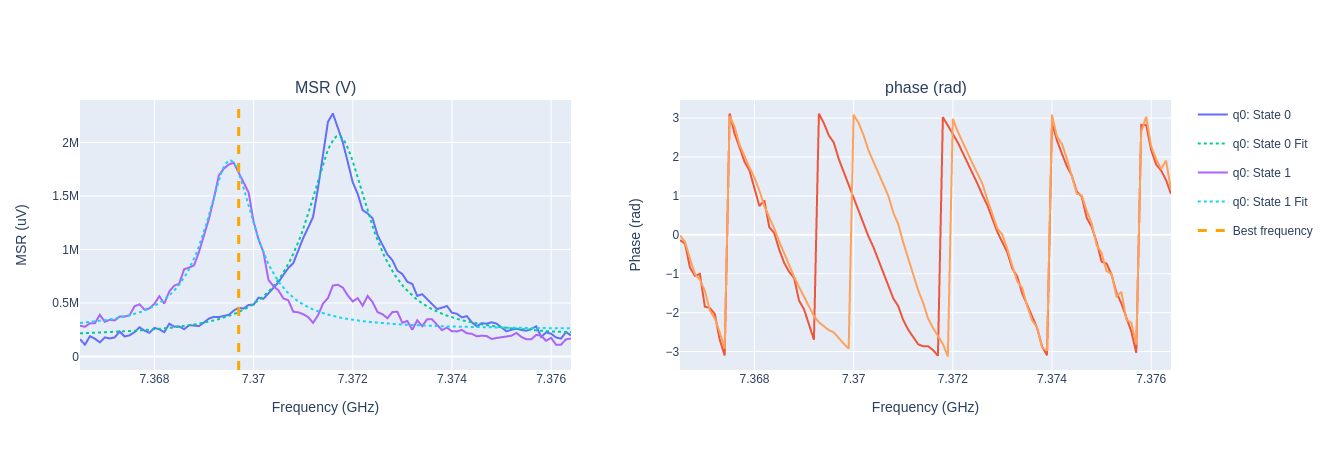
\includegraphics[width=1.3\textwidth]{characterization/figures/dispersive_shift.png}}
    \caption{Plot of a dispersive shift experiment.}
    \label{fig:dispersive_shift}
\end{figure}
As we can see in \cref{fig:dispersive_shift}, the optimal readout frequency does not correspond to the resonator peak for neither of these plots.

This experiment is just an ulterior optimization and is not strictly required, but can be used to improve the assignment fidelity.
Note also that, after a change in frequency for the measurement pulse, new classification parameters need to be computed.


\experimentrecap
{Readout optimization (dispersive shift)}
{readout calibration}
{optimized readout frequency,\\readout duration,\\dispersive shift}
{for the calibration of the pulse length, we try readout pulses with different length and choose the one that maximize the assignment fidelity. For the frequency, we perform a dispersive shift experiment: performing one resonator spectroscopy with the qubit in $\ket 0$ and one resonator spectroscopy with the qubit in $\ket 1$. We then choose the frequency that maximize the difference between the two states}




